\chapter{ISTTOK }

ISTTOK is a large aspect ratio tokamak (IPFN-IST, Lisbon, Portugal) operating for 30 years and which has been in constant upgrading of diagnostics, hardware acquisition system and control algorithms (major and minor plasma radius are respectively $R= 46 \, cm$, $a= 8.5 \, cm$). Together with the JT60-SA development of control techniques from last chapter, ISTTOK  studies  complement as a whole this work. This chapter will detailed how ISTTOK operates, from topics such as describing its diagnostics to description of the reconstruction method for calculating the plasma centroid position.

\section{Machine description}

The construction  of the actual ISTTOK machine was started in 1990 reusing some parts of the former dutch TORTUT tokamak: support structure, vacuum vessel, copper shell, toroidal magnetic coils, transformer, capacitor banks, radiofrequency (rf) generator, and discharge cleaning system ~\cite{Varandas1996}. The toroidal magnetic field is given by a set of 24 conventional coils which generate a maximum of 3~ T. The other components of ISTTOK such as the vacuum systems, the PF coils, and the power supply for the toroidal magnetic coils,  as well as its diagnostics and control and data acquisition system, were locally designed and built. Figure ~\ref{TopISTTOK} shows a top view of the ISTTOK tokamak and figure~\ref{ISTTOK_front} a frontal one in early 2020, its main elements are signalized with arrows.\smallskip

\begin{figure}[htbp]
	\centering
	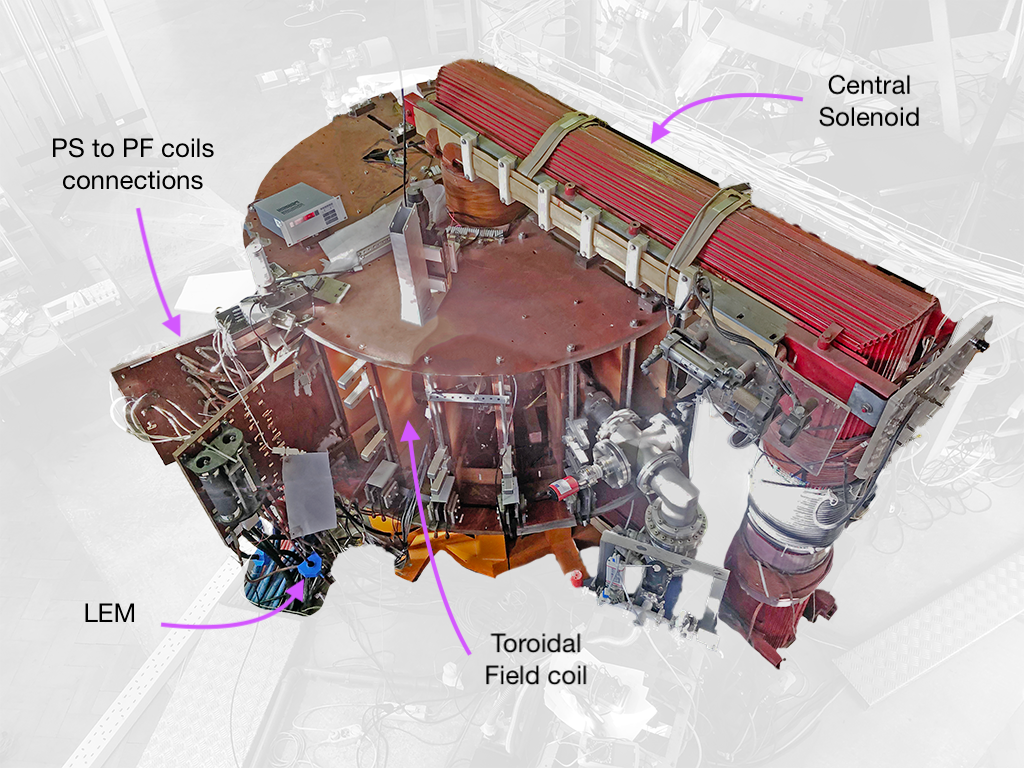
\includegraphics[width=1.1\textwidth]{Chp4/TopISTTOK.png}
	\caption{\label{TopISTTOK} ISTTOK top view in 2020,   main elements are indicated with magenta  lines.}
\end{figure}

\begin{figure}[htbp]
	\centering
	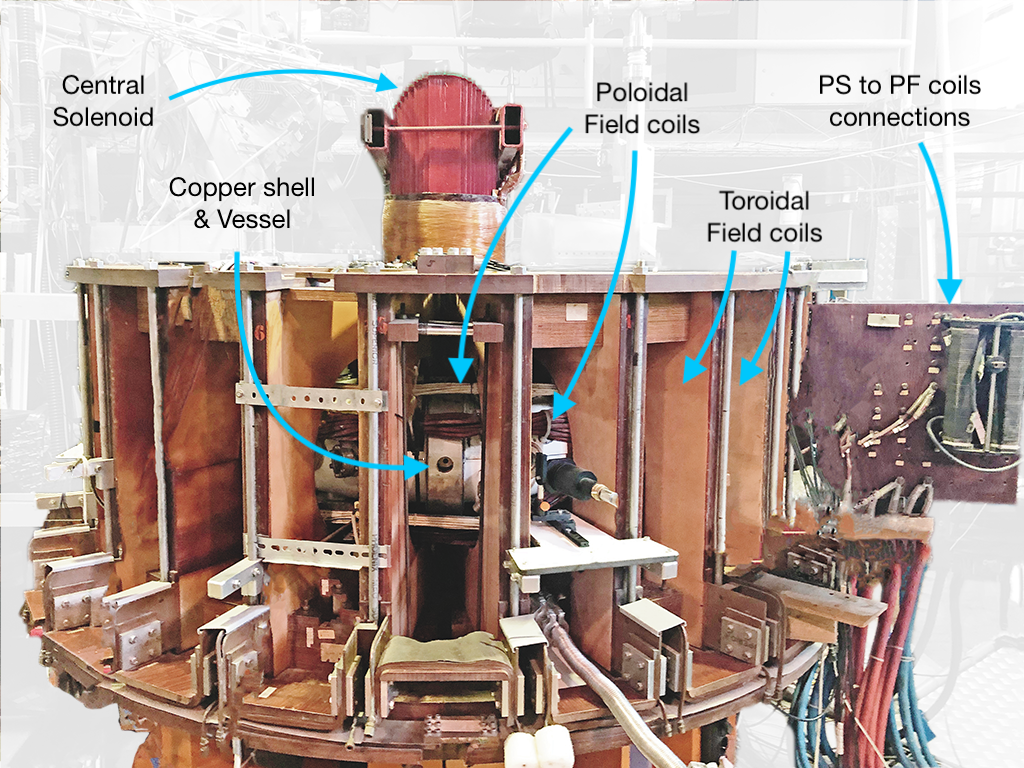
\includegraphics[width=1.1\textwidth]{Chp4/FrontISTTOK.png}
	\caption{\label{ISTTOK_front}ISTTOK frontal view in 2020, main elements are indicated with blue lines.   }
\end{figure}

Figure ~\ref{VV_IST} corresponds to a section of the ISTTOK vacuum vessel, it is possible to observe on the image the ribbed  surface from the vessel and some of the ports on the top of it. The vacuum vessel is formed by two half torus made of INCONEL alloy 625 with a thickness of 0.15~ mm. The vacuum vessel is completely surrounded by a 1.5 ~cm thick cooper shell which is possible to see in the images from figure~\ref{ISTTOKviews}, this shell supports the vacuum vessel and it originally  also worked suppressing  variations of the plasma position in less than 2~ms since a first version of TORTUR had no PF coils, this was a form of auto-control. The  cooper shell, due to its properties, adds a delay or skin time for the  penetration of the magnetic fields into the vacuum vessel.
\smallskip

\begin{figure}[htbp]
	\centering
	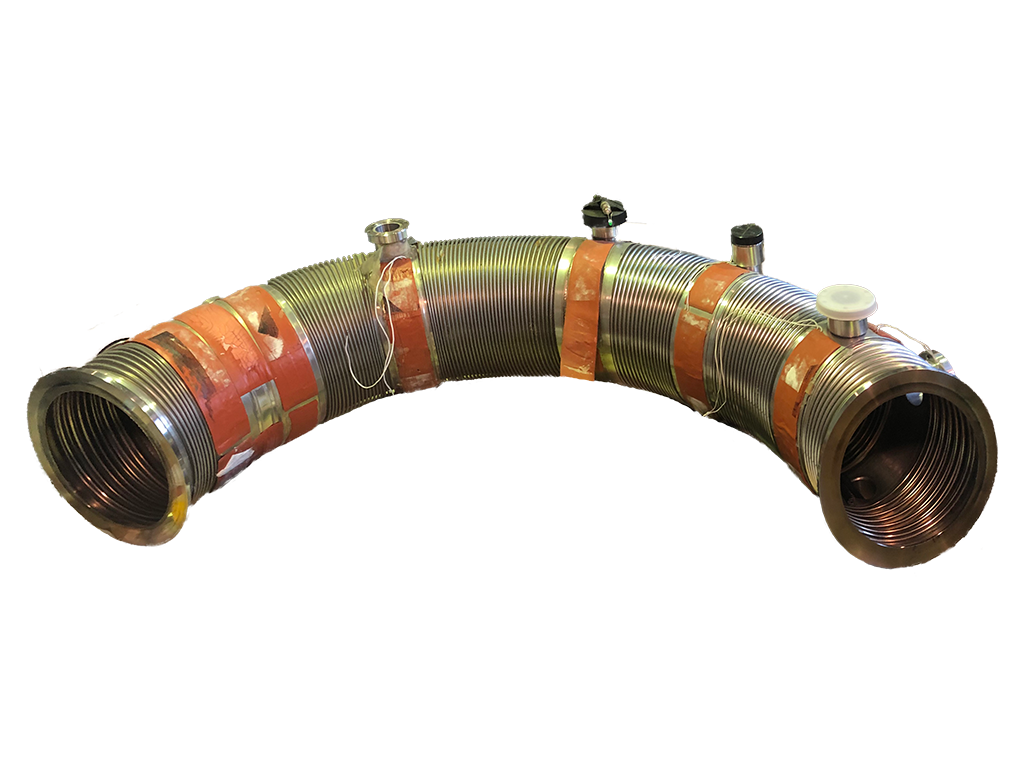
\includegraphics[width=0.65\textwidth]{Chp4/VacuumVessel_Low.png}
	\caption{\label{VV_IST} Actual ISTTOK inconel  vaccum vessel section with ports.  }
\end{figure}





\subsection{ISTTOK AC plasma current}


The STOR-M tokamak was the first device to demonstrate an alternation in the plasma current even though the control position for negative cycles was not very successful ~\cite{Mitarai1996}, afterwards in JET, plasma current reversal was implemented as a necessity to demonstrate the feasibility of AC operation in conditions which can be considered relevant to a reactor achieving plasma current of 2~MA in each direction along with modifications in the PF coils powers supplies control systems ~\cite{Tubbing1992}.\smallskip

One of the main characteristics from ISTTOK  is that due to the flexibility of the power supplies it is possible  to perform  AC  discharges  which  allow the fast reversal of the plasma current while maintaining a finite plasma density between consecutive flat tops  ~\cite{density}. The current inversions make it possible to achieve a much longer plasma duration in comparison to single mode operation, which is limited by the saturation of the iron core magnetization,the plasma duration is of approximately 1 s with positive and negative flat-tops of $\approx 25~ms$ (~\cite{Fernandes1998}, ~\cite{Carvalho2015}~). An AC plasma current also accounts for  an inversion in the direction of the poloidal magnetic field, from the equation ~\ref{force_balance} is possible to see that a change of sing in the poloidal field $B_\theta$ while the toroidal field $B_{\phi}$ remains the same only implies a change of sign in the required vertical field for achieving toroidal force balance. ISTTOK has dwell time in between positive and negative cycles of $\approx 1~ms$.\smallskip


\section{Diagnostics and Actuators}

Different  diagnostics are integrated in ISTTOK to retrieve important plasma parameters, i.e. langmuir probes, tomography, magnetic probes. This work is focused on the magnetic diagnostics  since they are responsible for  retrieving the signals necessaries to reconstructed the centroid position of the column and the plasma current. ISTTOK has a set of 12 of magnetic  probes or Mirnov coils positioned along the poloidal direction (30° between  probes), each coil has an area of $49 ~mm^2$ , 50 turns and a length of 5 ~mm, a scheme is depicted in figure ~\ref{MirnvC}. Picture from figure ~\ref{MirnPort} shows the vessel side port where the magnetic probes are  placed and its acquisition cables along with some of the PF coils cables in orange and white. Each coil is inside a graphite box and the set of 12 forms the plasma limiter, see figure \ref{MirnvC_photo} and ~\ref{limiterBox}. Magnetic probes send an induced voltage given by Faraday's law $~\varepsilon = -N\frac{\Phi_P}{dt}$ where $\Phi_P$ is the poloidal magnetic flux generated by the plasma and passive elements passing through the probe cross-section.
\smallskip



\begin{figure}
	\centering
	\begin{subfigure}[b]{0.37\textwidth}
		\includegraphics[width=\textwidth]{Chp4/MirnovCoil_locations_ISTTOK.eps}
		\caption{ Set of 12 magnetic probes for the reconstruction of the plasma centroid position located along the poloidal direction at ISTTOK.\label{MirnvC} }
	\end{subfigure}
	~~
	\begin{subfigure}[b]{0.37\textwidth}
		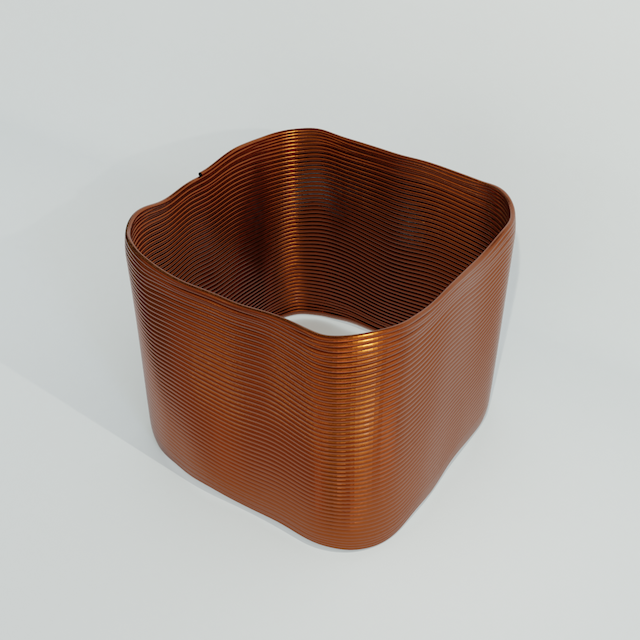
\includegraphics[width=\textwidth]{Chp4/mirn_coil.png}
		\caption{\label{MirnvC_photo} 3D model of ISTTOK magnetic probe coil, each probe is capsuled inside a graphite box cut horizontally to avois eddy-currents. }
	\end{subfigure}
~~
		\begin{subfigure}[b]{0.37\textwidth}
		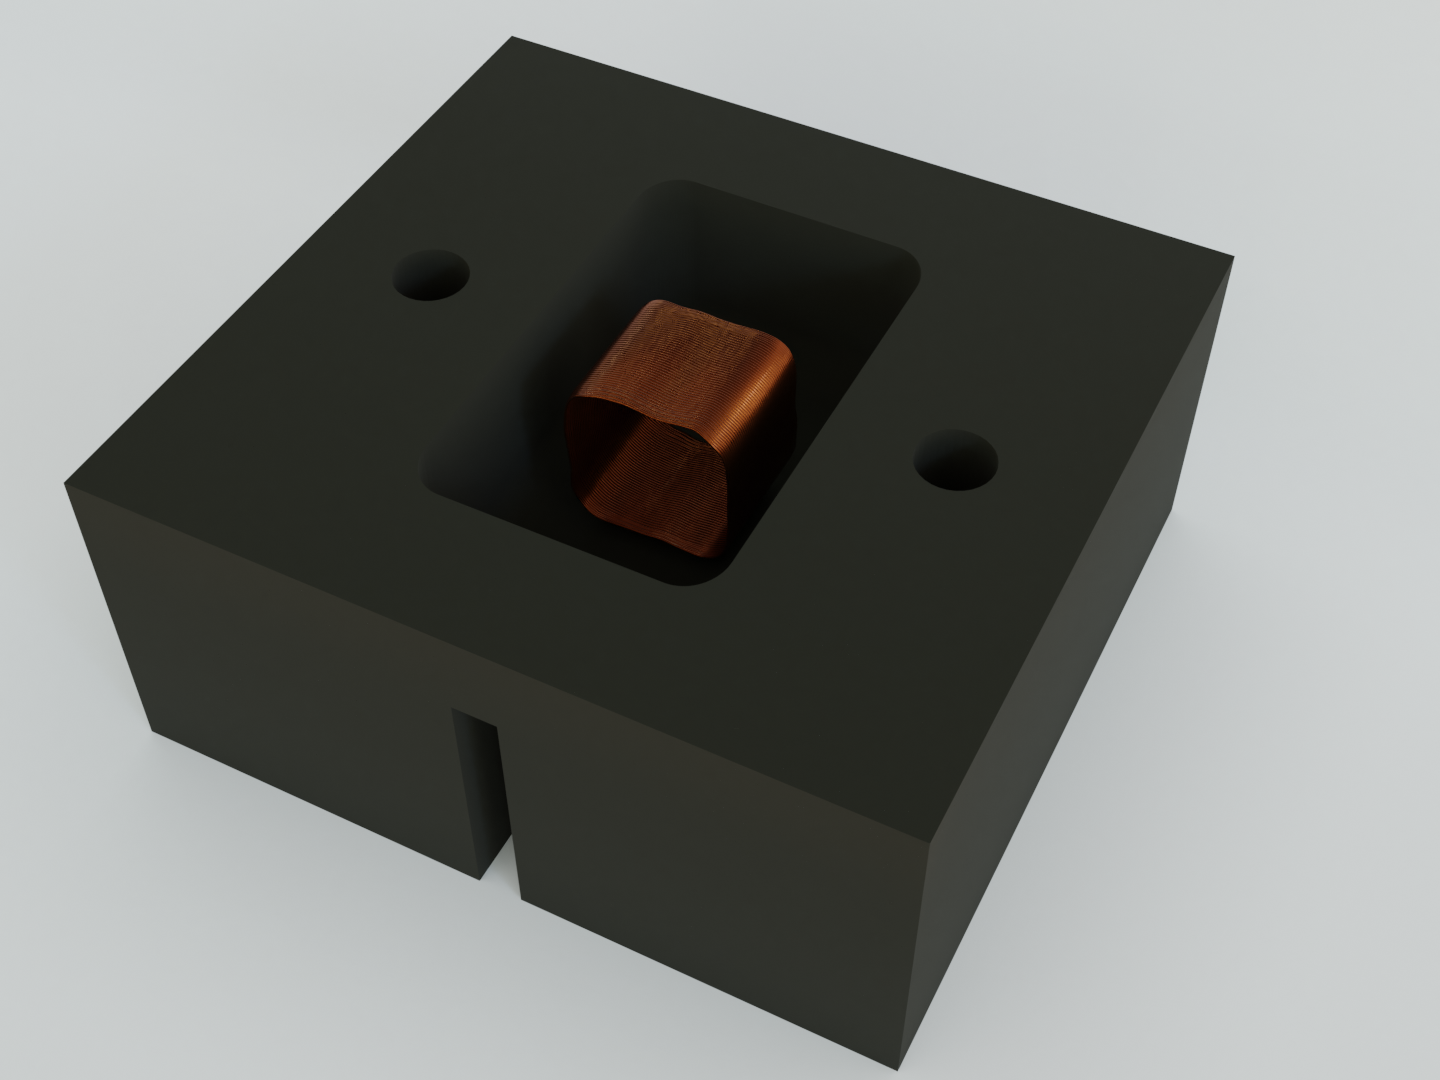
\includegraphics[width=\textwidth]{Chp4/limiterBox.png}
		\caption{\label{limiterBox} 3D model of one graphite box which conforms the limiter and contains a magnetic probe inside. Traversal edges in the box avoid the presence of eddy currents.   }
	\end{subfigure}
	\caption{ ISTTOK magnetic probes.\label{all_mirnv} }
\end{figure}



A second set of diagnostics important for this work are the three current transducers, also called LEMs, installed in ISTTOK for measuring the current applied by the power supplies  to each  PF coils, figure ~\ref{LEM} show a picture of one LEM.

\smallskip


\begin{figure}[htbp]
	\centering
	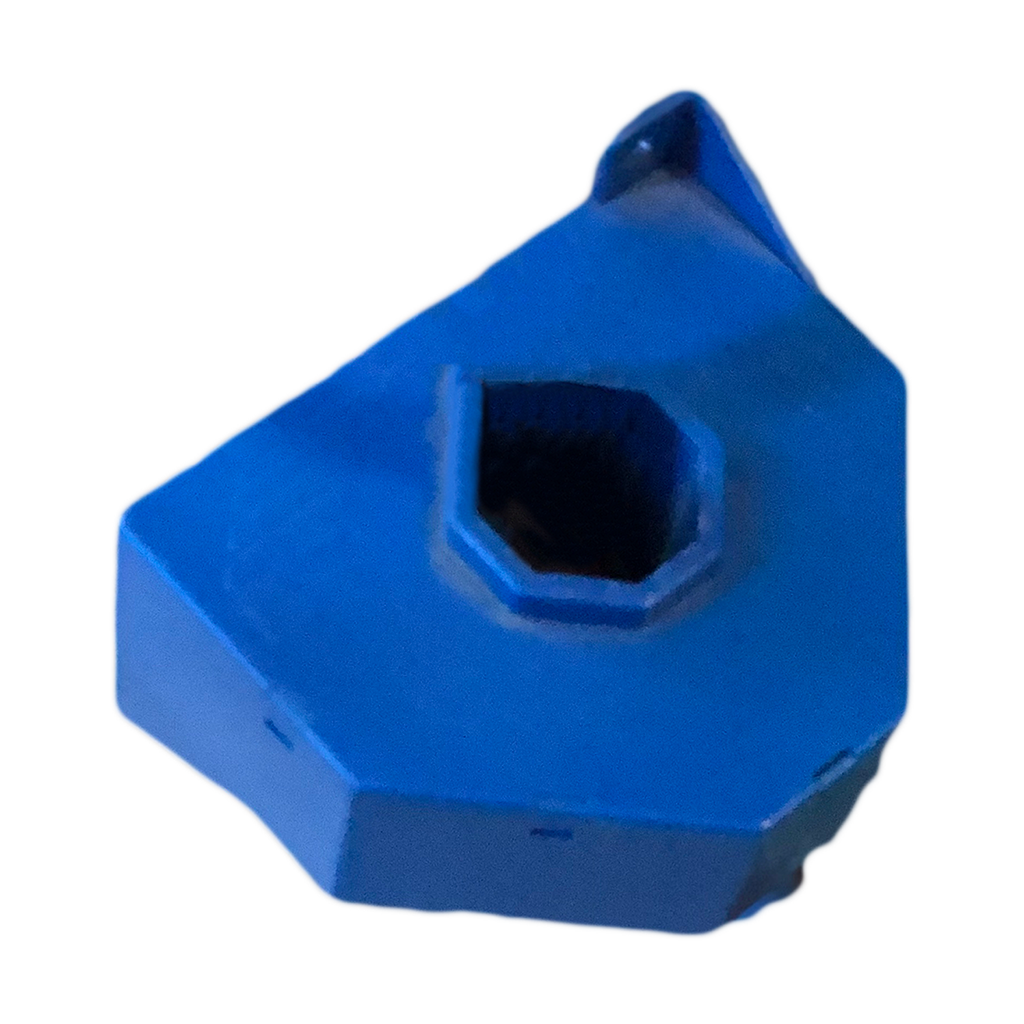
\includegraphics[width=0.4\textwidth]{Chp4/LEM.png}
	\caption{\label{LEM} LEM transducer for measuring the current from the power supplies to the PF coils.  }
\end{figure}

\begin{figure}
	\centering
	\begin{subfigure}[b]{0.37\textwidth}
		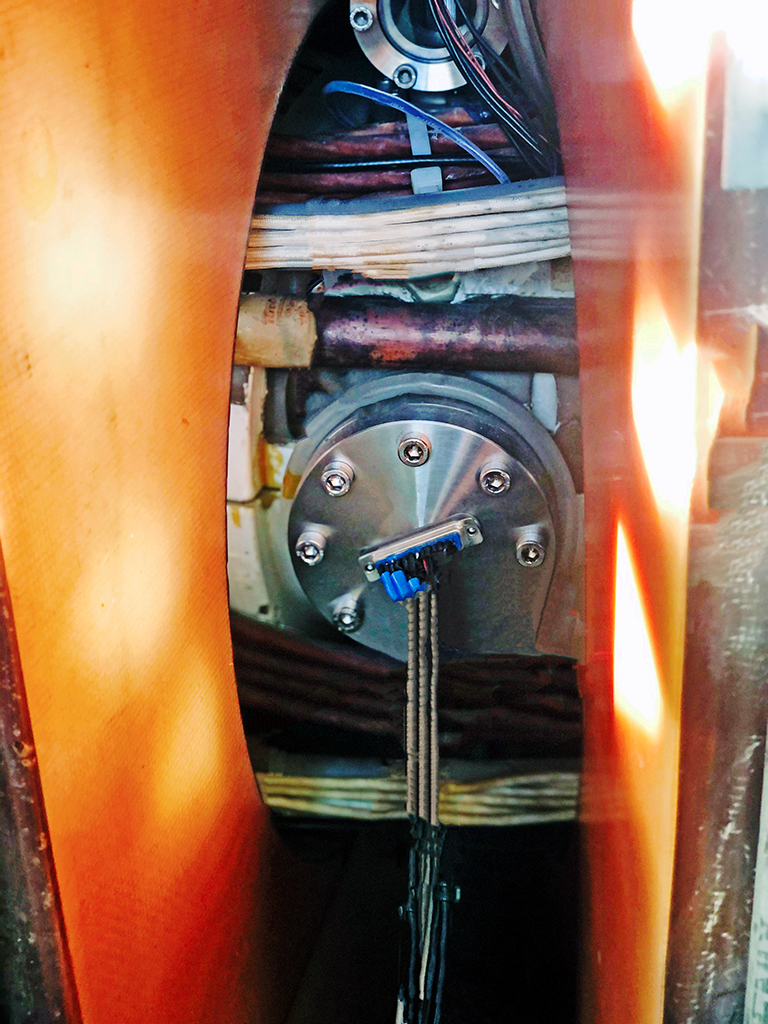
\includegraphics[width=\textwidth]{Chp4/PuertoMirnov.png}
	\caption{\label{MirnPort}Magnetic probes port with connection cable to the ATCA acquisition boards, also PF coils and cooper shell are shown. }
	\end{subfigure}
~~~~
	\begin{subfigure}[b]{0.37\textwidth}
		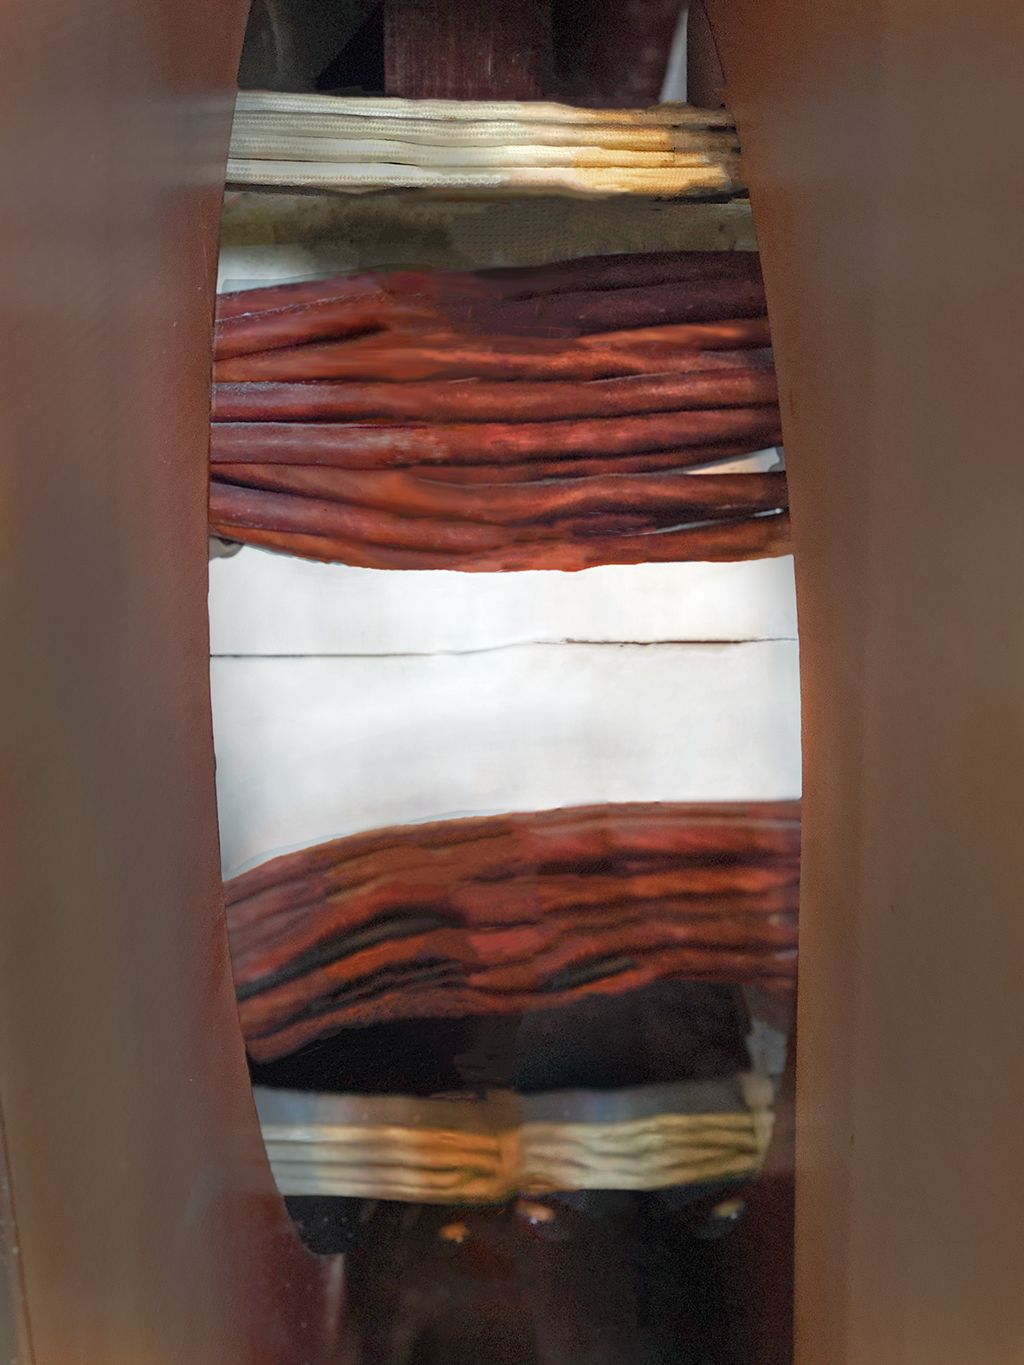
\includegraphics[width=\textwidth]{Chp4/PFCoils.png}
	\caption{\label{ISTTOKpfCoils}PF coils close up,primary coils correspond to the  white cables and vertical and horizontal to the orange ones. }
\end{subfigure}

 \caption{ISTTOK close up side views. \label{ISTTOKviews} }
 
 
\end{figure}

\subsection{Poloidal Field Coils}

ISTTOK poloidal field coils are placed in between the TF coils and the cooper shell. In figures ~\ref{MirnPort} and ~\ref{ISTTOKpfCoils} is possible to see the cables from the PF coils arrange in sets of orange and white cables. ISTTOK Poloidal Field (PF) coils are connected to three independently feedback controlled power supplies for the purpose of generating plasma current and also to control vertically and horizontally its centroid position. In figure~\ref{PF_coils} is shown on the right side of the iron core an  old central solenoid which used to be responsible for plasma current generation, this element is currently disconnected.  The primary PF coils, in white color, generate ohmic heating for the creation of plasma current and an additional vertical field. In yellow is depicted the vertical PF coils and in green the horizontal PF coils, both controlled by different control algorithms in order to follow a centroid position set point \cite{IvoPID}. The PF coils power supplies have as saturation limits $I_{sat-prim}=\pm~ 300~A$, $I_{sat-vert}=\pm~ 400~A$ and $I_{sat-hor}=\pm~ 200~A$. Figure ~\ref{PF_lines} shows the magnetic field lines generated by each PF coil around the vacuum chamber cross section on their nominal positions:\smallskip

$\bullet$ Primary PF coils: 2 coils, 14 turns,($R_{1,2}=62 ~cm~,~z=13 ~cm\pm$).
\smallskip

$\bullet$ Vertical PF coils: 4 coils, 5 turns,($R_{1,2}=58 ~cm~, R_{3,4}=34 ~cm ~z=7 ~cm\pm$).
\smallskip

$\bullet$ Horizontal PF coils: 2 coils, 4 turns,($R_{1,2}=58 ~cm~, ~z=7 ~cm\pm$).
\smallskip

%% Aqui va la figura de Dori
\begin{figure}[htbp]
	\centering
	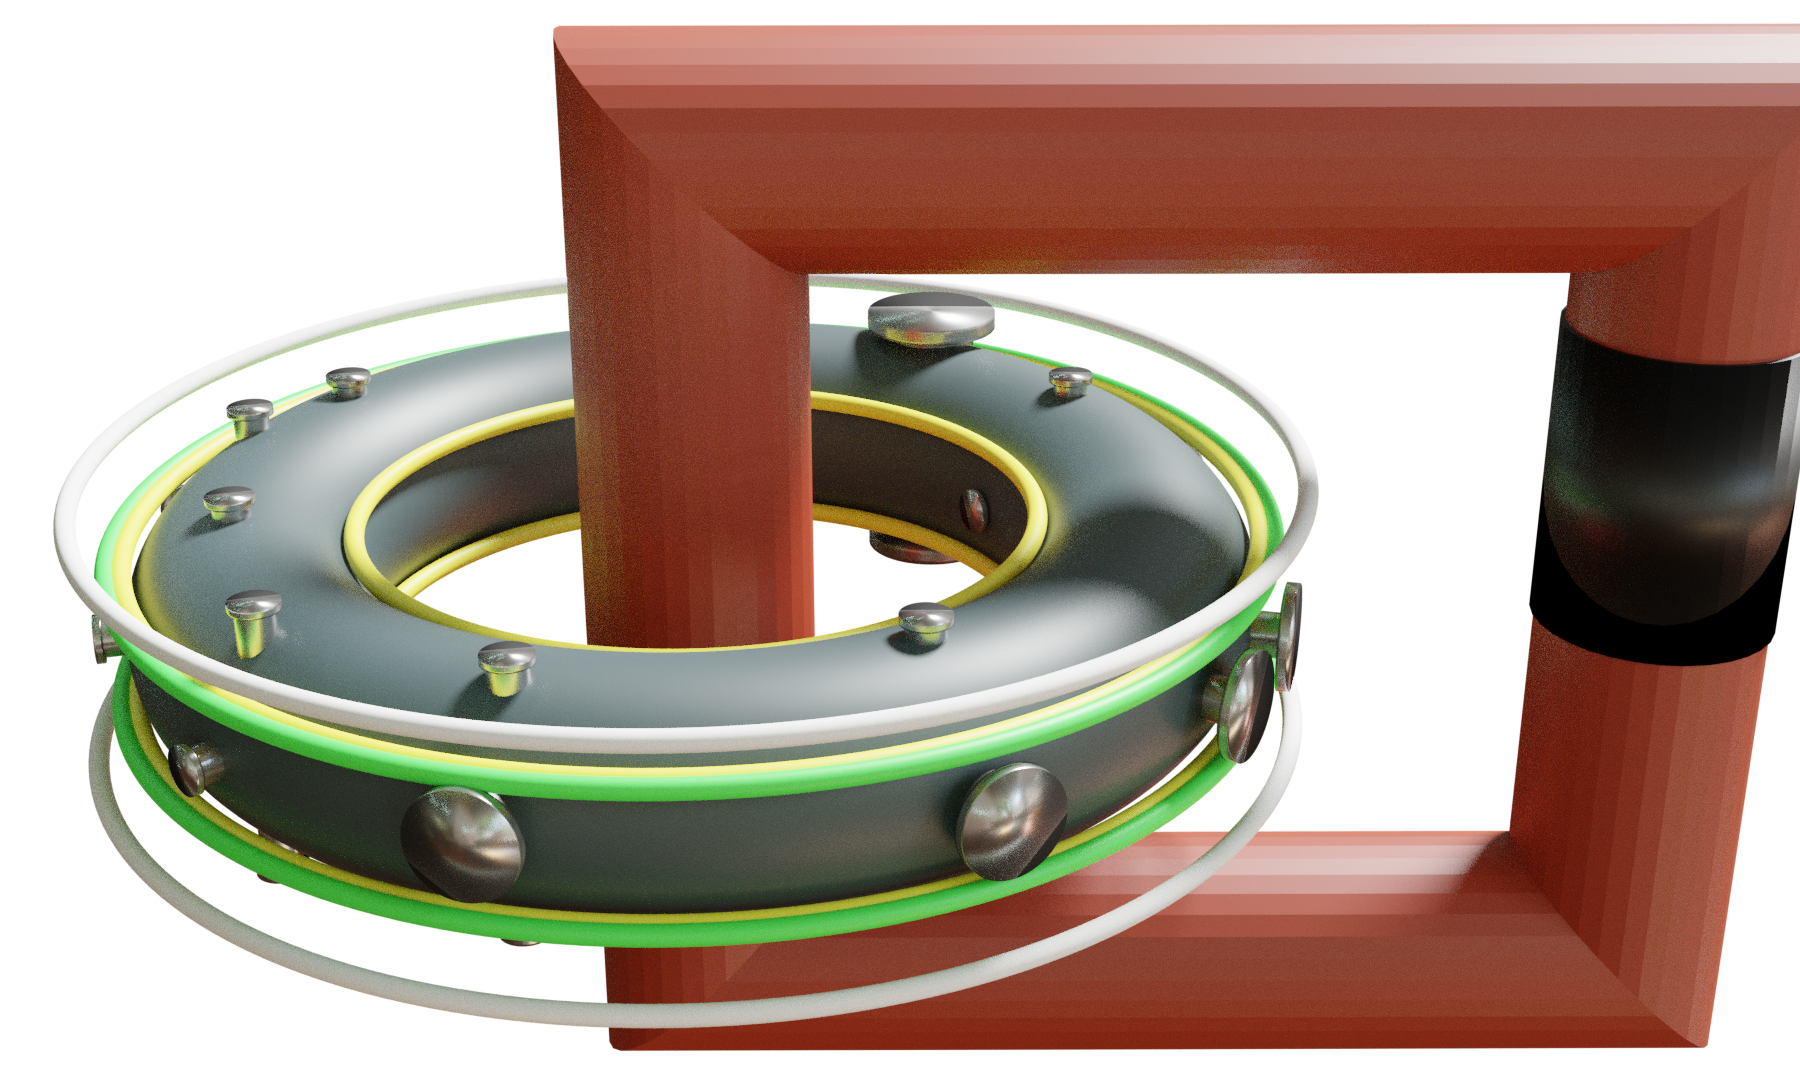
\includegraphics[width=0.9\textwidth]{Chp4/ist_coils.png}
	\caption{ 3D model of the ISTTOK PF coils, vacuum chamber with ports, iron core and the former central solenoid (black color). Primary coils (white color) and horizontal coils (green color) are formed by 2 coils each one and located on the  upper and lower LFS (Low Field Side) of tokamak. Vertical coils (yellow color) are formed by 4 coils, 2 are located on the upper and lower LFS and 2 in the upper and lower HFS (High Field Side). \label{PF_coils}  }
\end{figure}

\begin{figure}[htbp]
	\centering
	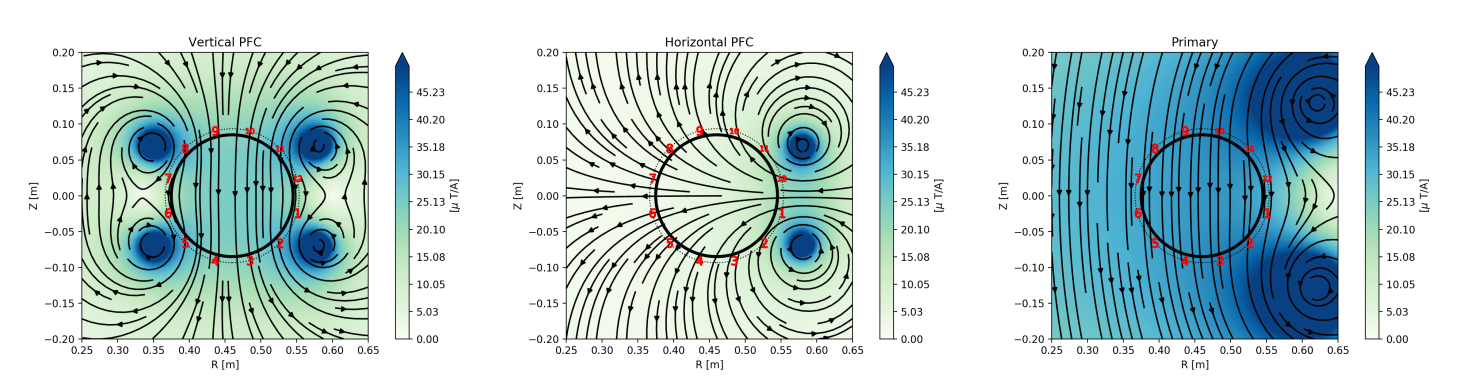
\includegraphics[width=1.12\textwidth]{Chp4/PF_fieldLines.png}
	\caption{ Magnetic field generated by the active coil circuits on their nominal positions. Mirnov positions are represented by its sequential number (in red) over the dashed line. Black circle represents the limiter.\label{PF_lines}  }
\end{figure}


%The ohmic heating (OH) coils of the tokamak transformer,
%Since the ISTTOK central solenoid is not being used as the primary winding to create the toroidal electric field responsible for creating and maintaining the plasma current  $I_p$ ,

As mentioned before, figure~\ref{PF_coils} shows the  nominal positions of the PF coils. From the pictures in figure~\ref{ISTTOKviews} is notorious that specially the vertical and horizontal PF coils (orange cables) are not uniformly arranged, toroidally not very axisymmetric and they seam to have a general negative offset in the vertical coordinate, on top of that there is no certain notion of how the internal vertical coils have moved through the years, this represented and issue  attempting to adjust a theoretical ISTTOK model based on the CREATE codes.\smallskip





\section{ISTTOK Hardware }

ISTTOK real-time control diagnostics and actuators  implementation rely  on the recently upgraded hardware based on the Advanced Telecommunications Computing Architecture (ATCA).   The real-time control system is programmed on top of the Multi-threaded Application Real-Time executor (MARTe) framework,  which  integrates and processes the information gathered by all the  diagnostics \cite{Ivo2}, figure ~\ref{ISTTOK_hard} depicts the schematic of the implemented control system at ISTTOK.

\begin{figure}[htbp]
	\centering
	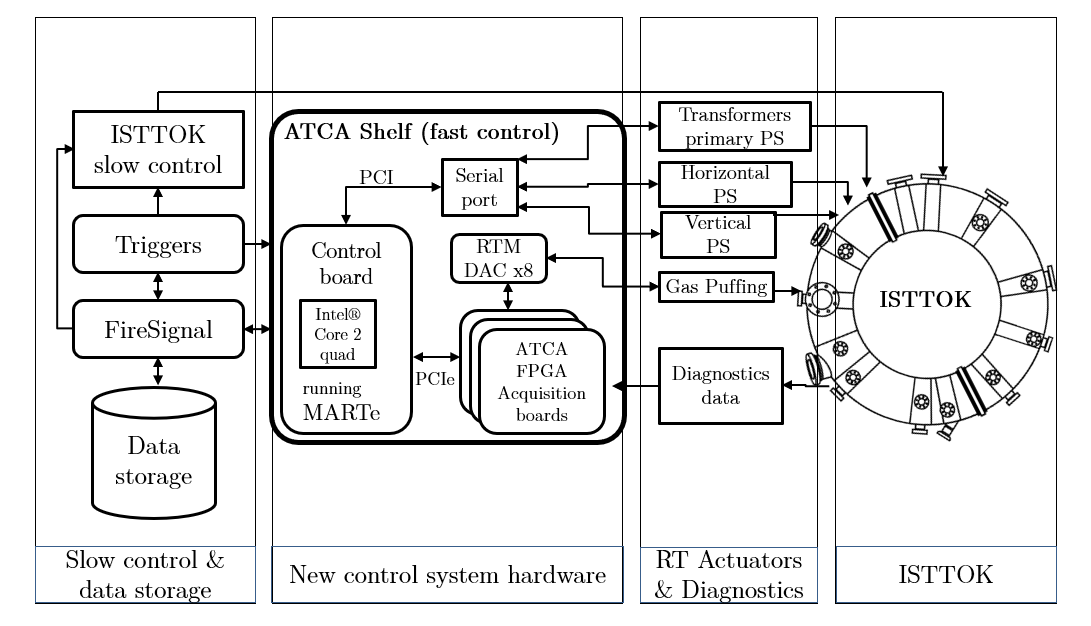
\includegraphics[width=0.85\textwidth]{Chp4/control_schem_1.PNG}
	\caption{\label{ISTTOK_hard} ISTTOK hardware overall scheme. Data is acquired by the
		ATCA data acquisition boards, and decimated and transferred to the hosts
		every 100 $~\mu s$. }
\end{figure}


Recently implemented hardware-integrated acquisition of the magnetic probes signals at ISTTOK allowed the implementation of new real-time algorithms for an accurate reconstruction of the current centroid position. \smallskip

\subsection{ATCA-MIMO-ISOL boards}

The ATCA carrier board, already slightly address in chapter ~\ref{Chap2}, is an IPFN developed board ~\cite{Batista2010} complying with the ATCA standard specification, highly modularized, and with an optional Rear Transition Module (RTM) . The carrier board can hold up 32 analog input channels, each connected to a plugged-in ADC module. All modules are connected digitally to a XILINX Virtex-4 FPGA which performs necessary digital signal processing and includes a PCI Express Endpoint providing the data interface to the ATCA switch board. Figure ~\ref{ATCA_ISOL} shows a newer version   from the board in figure ~\ref{PCIe}, both share basically the same elements. The latest version of the ATCA-MIMO-ISOL boards built in IPFN where mainly intended for the magnetic acquisition in the stellerator W7-X and lately tested in ISTTOK.  
\smallskip




\begin{figure}[htbp]
	\centering
	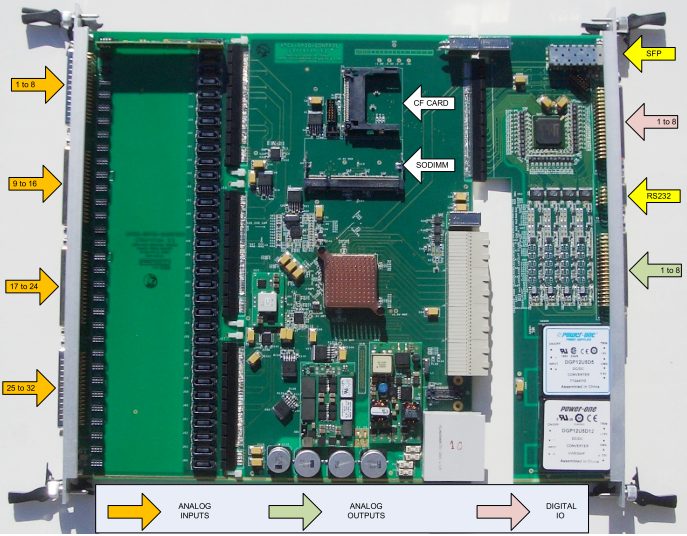
\includegraphics[width=0.85\textwidth]{Chp4/ATCA_MIMO_ISOL.png}
	\caption{\label{ATCA_ISOL} General view of the ATCA-MIMO-ISOL carrier board, including on the right side an original IPFN RTM board joined through an edge connector. }
\end{figure}

The phase modulated (chopper) ADC module~\cite{Batista2010} was designed targeting the digital integration of signals generated by magnetic coils, over periods of time larger
than one hour. This ADC module is composed by a  Signal Condition block with a passive filter attenuator and an active differential amplifier, the ADC block (18-bit resolution, fixed 2MSPS (Mega samples per second)), a DC-DC converter and a Magnetic Isolation coupler (ILS711-S1) and finally the digital interface to the FPGA in the ATCA carrier Board. The FPGA also provides the clock signals for the DC-DC converter, the chopper and ADC clock (common to all channels) and receives the serial ADC data and respective clock signals.




\section{Real-time  integration software}

To recover the magnetic fields absolute magnitude from inductive probe signals an integrating component is needed. Typical analog electronic integrator circuits always suffer from voltage offsets and drifts present in the components and wiring. Even very low offsets integrated during a long period of time may appear as a noticeable deviation of the integrated signals ~\cite{Spuig2003} and eventually saturate their outputs. A solution chosen for this integrator design, previously demonstrated in a four channel prototype in PXI format ~\cite{Werner2008}, was to modulate signals with a phase invertor (chopper), which reverses periodically the input signal before active amplification ( multiplies the signal by 1 and then by -1), filtering and sampling in the ADC, as shown in figure ~\ref{ADC_FPGA}. The switching frequency is programmable and made synchronous with the sampling ADC 2Mhz clock, as both are generated in the same FPGA. By applying the signal inversion before any electronic amplification, and reconstructing the digital equivalent of the signal after the digitalization, the average of the electronics offset (EO) is expected to be almost  zero in the integration process if its value is steady enough over at least two inversion periods. In addition a second offset also appears before the chopper, the Wiring offset (WO) which may be generated either inside the module or in the external wiring, connectors and soldered parts, mainly due to uncompensated thermocouple effects, external interference or radiation effects. Unfortunately,the WO is not averaged by the chopping method, since it goes across two signal reversions, and is typically much lower than either both EO or the ADC resolution, the process for removing the WO in real-time will be discussed ahead. From figure ~\ref{ADC_FPGA} the integration process can be inferred. Let's say the upcoming signal from the probe is $s(t)$, the sampled value is $V_{ADC}[n]$ and $t=nT_s$, where $T_s$ is the ADC sampling period:
\smallskip


\begin{figure}[htbp]
	\centering
	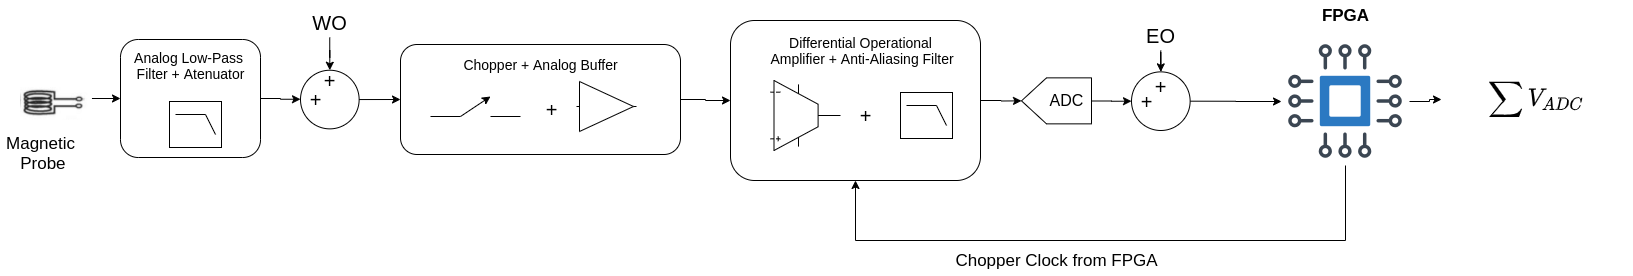
\includegraphics[width=1\textwidth]{Chp4/ADC_FPGA.png}
	\caption{\label{ADC_FPGA} ADC module diagram depicting the influence of the WO and EO offsets and the instrumentation since the magnetic probes signal it is acquired until its integration in the FPGA. }
\end{figure}

\begin{equation}
V_{ADC}=(s(nT_s)+WO)\cdot Ph_{chop}(nTs)~+~EO \qquad \textbf{V}
\end{equation}
where $Ph_{chop}$ is the phase signal of the chopper (1 or -1). Assuming $s(nT_s)\approx n[T]~$and$~Ph_{chop}(nT_s)\approx Ph_{chop}[n] $, the phase reconstructed signal from the magnetic probe can thus be approximated from the discrete samples using:
\begin{equation}
s[n]~\approx (V_{ADC}-EO) \cdot Ph_{chop}[n]~-~WO\qquad \textbf{V}
\end{equation}

Assuming the ADC sampling frequency is sufficiently higher than double of signal bandwidth, the integral related to magnetic fluxes can then be approximated by the expression:
\smallskip
 \begin{equation}
 	\Phi (t=nT_s)=\int_{0}^{t=nT_s} s(t)dt~\approx \sum_{0}^{N} ((V_{ADC}[n]-EO)\cdot ~ Ph_{chop}[n])~-~nT_s\cdot Wo\qquad \textbf{V } \cdot \textbf{s}
 \end{equation}

Thus, the $V_{ADC}$ summation for approximating the integral of the signals acquired from the magnetic diagnostics is computed  in the FPGA and then sent to the MARTe database via PCI-express.\smallskip
 

Even tough  WO removal is a common feature in processing magnetic data it is remarkable the flexibility ISTTOK gives by allowing the calculation of the offset prior to each discharge. In contrast with other experiments where the offsets do not tent to change and have to be calibrate one single time, due to the physical conditions in ISTTOK the offset values are in constant change and so they should be calculate on real-time prior to  every discharge.Figure  ~\ref{WO_percent} shows the WO percentage change in the magnetic probe $\#$ 10  in 2019, it is possible to observed that in most of the shots the changing percentage is of at least $\approx~30\%$, figure   ~\ref{WO_minr10} shows the WO values and percentage changes for a less number of shots on the magnetic probe $\#10$, this shot numbers correspond to data acquisitions where the WO had the smallest changes, from these figures is possible to conclude that is needed a real-time algorithm to calculate the WO on each probe prior to a plasma discharge. \smallskip

\begin{figure}[htbp]
	\centering
	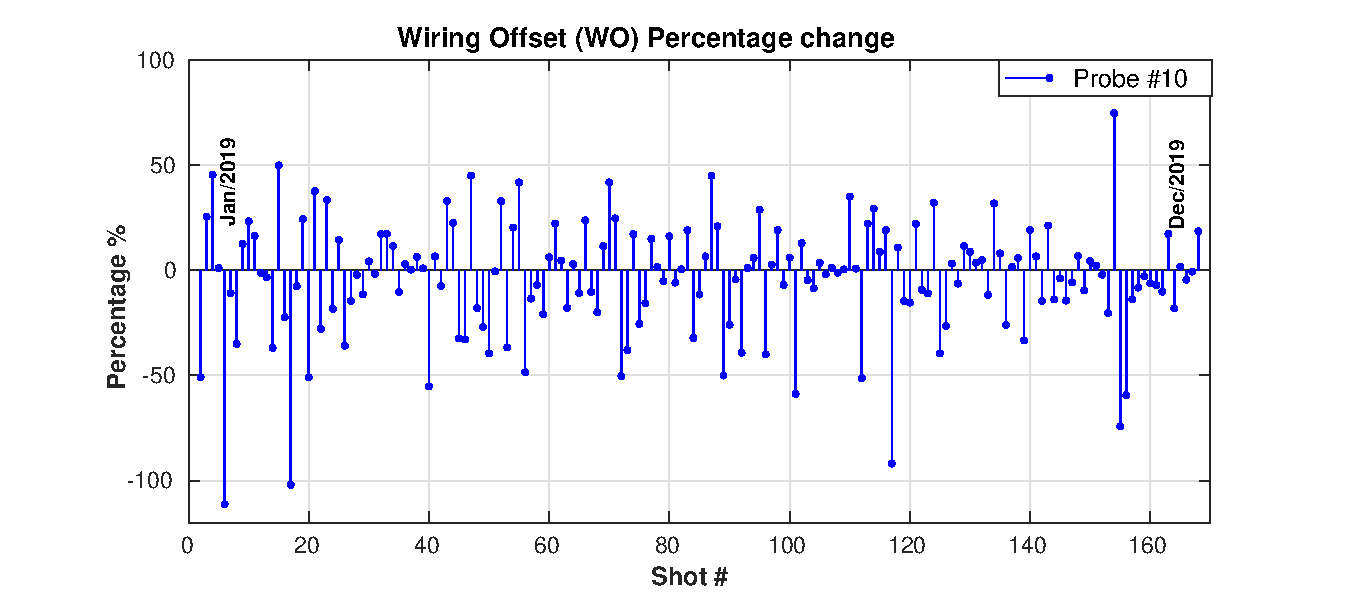
\includegraphics[width=0.85\textwidth]{Chp4/percentage_change.eps}
	\caption{\label{WO_percent} WO percentage change in the magnetic probe $\#$ 10  in 2019 using data from approximately  180 shots distributed during the entire year. }
\end{figure}

\begin{figure}[htbp]
	\centering
	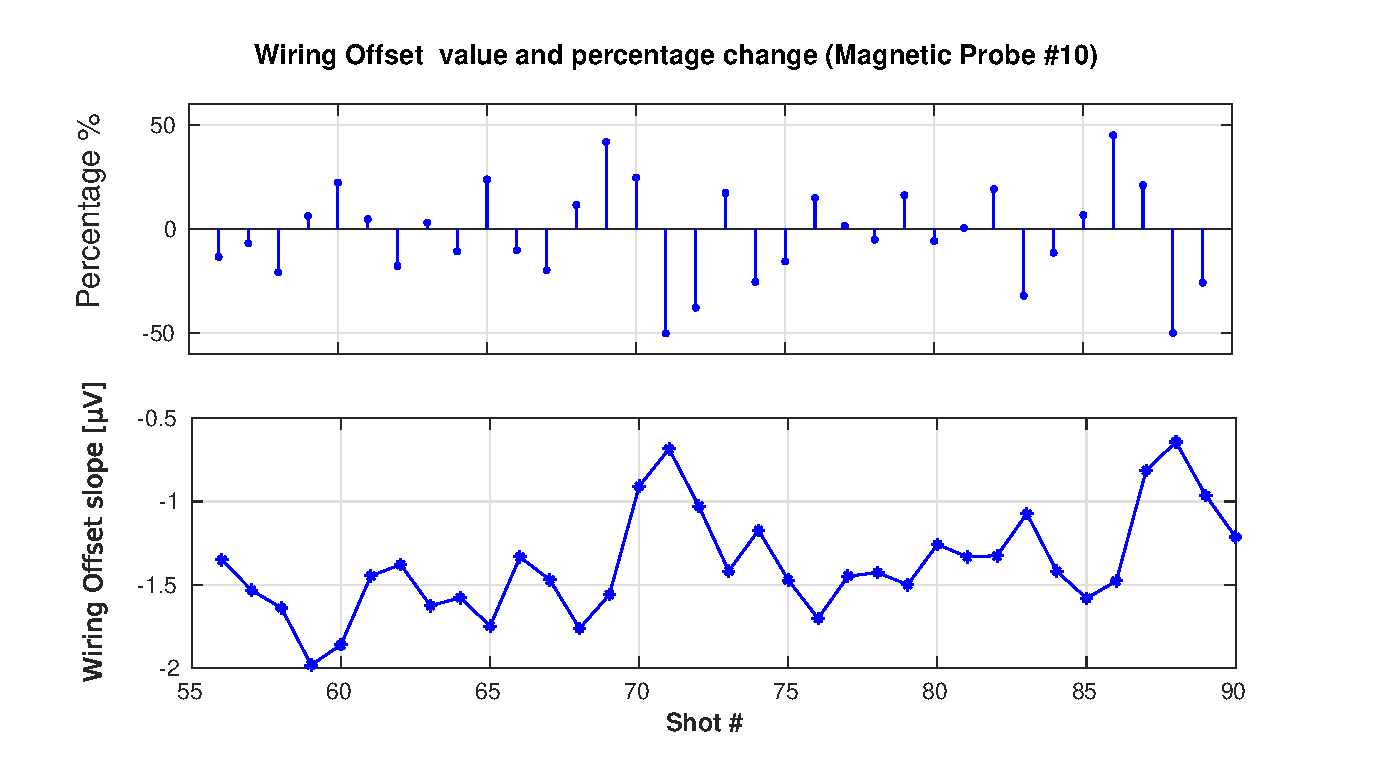
\includegraphics[width=0.85\textwidth]{Chp4/valueAndpercentage_change10.eps}
	\caption{\label{WO_minr10} WO and percentage change in the magnetic probe $\#4$  throughout 45 shots in ISTTOK.}
\end{figure}

 At ISTTOK it is possible to acquire data using the MARTe framework. Even thought the probes signals before the discharge starts are not  stored on the data base, this feature allows to compute the WO of each probe several seconds before the discharge starts. For this process a GAM stores the signal from each integrated magnetic probe and calculates the slope from $t=0$ until $t=1~s$, repeats this process every second during  30~s and calculates an average WO value for each coil. The WO  value obtained  is then subtracted on every MARTe iteration once the discharge starts from the actual probe signals.   In  figure ~\ref{offset_remove} it is possible to observe the integrated WO summed to the probe signal.  \smallskip

\begin{figure}[htbp]
	\centering
	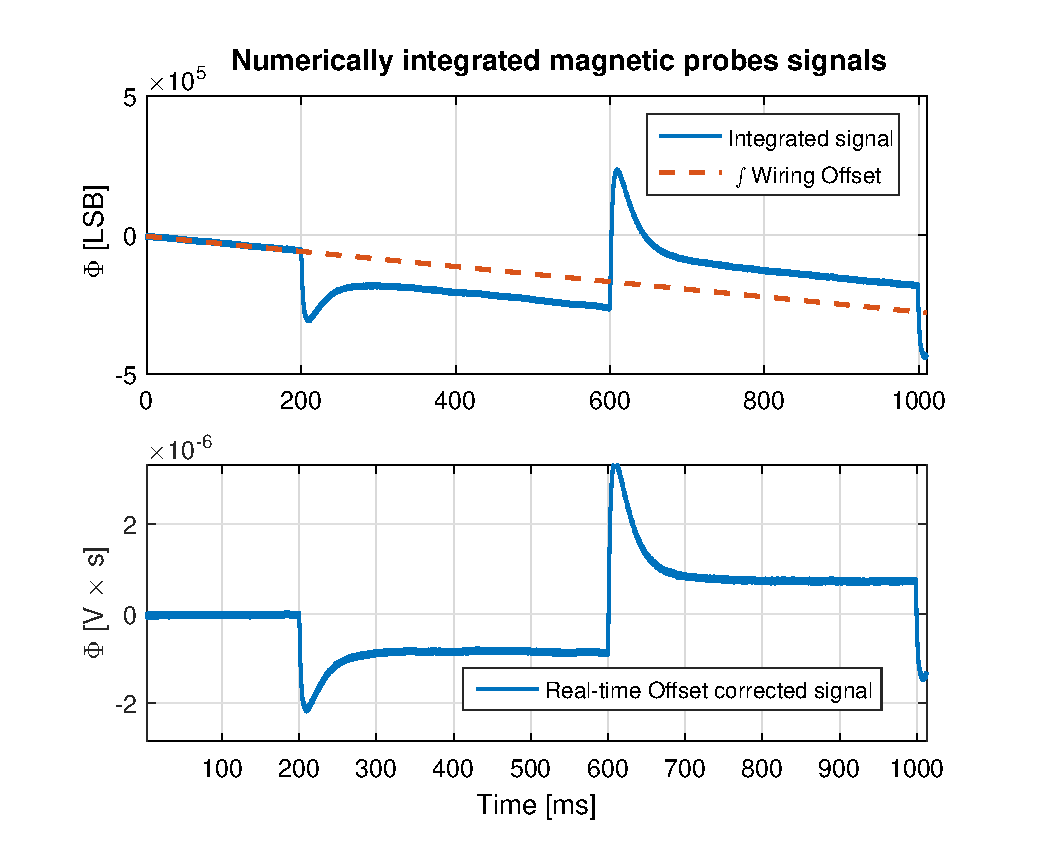
\includegraphics[width=0.6\textwidth]{Chp4/offset_remov_1}
	\caption{\label{offset_remove} Real-time subtraction from the integrated WO is performed on every MARTe cycle for each magnetic probe.  }
\end{figure}

%
%Several design variants of the chopper-based digital signal integrators were tested to evaluate the optimal solution to achieve the ITER magnetics diagnostic requirements for further down the line \cite{Batista2018}.
%\smallskip


\section{Plasma current magnetic field }

Retrieving the magnetic contribution of the plasma current in tokamaks can be achieved through the integrated magnetic probes signals. The magnetic probes are exposed to any poloidal field present in their surrounding which are: poloidal field generated by $I_p$, poloidal field generated by the PF coils and field generate by the eddy currents in the passive structures. Reconstructing the plasma centroid position from the signals in the magnetic probes implies that a process should be perform in order to extract only the plasma current magnetic contribution to the probes.  On this section the methods of correction of the magnetic external fields due to PF coils, inaccuracies of tokamak manufacturing and assembly are considered. \smallskip


\subsection{PF coils state-space model estimation}

 Since currently the PF coils positions are not similar to the nominal ones and due to its physical configuration is hard to measure their positions and clearly identify the cables from each coil, the attempts to create a theoretical model for ISTTOK did not succeeded. Even though this fact could have brought a barrier for characterizing ISTTOK, this situation allowed to use different approaches and apply computational tools never used  in order to implement novelty deployments in ISTTOK.   \smallskip

Performing plasma-less discharges in ISTTOK by applying different step functions waveforms in the PF coils currents,  data-driven discrete state-space models were obtained in order to determine the contribution to the probes signals from passive-structures eddy currents and PF coils fluxes at any instant. Due to the linear dynamics of the PF coils and the simplicity for implementing the state-space equations on top of MARTe framework it was decided to use state-space models for the reconstruction of external contributions \cite[Chapter~2]{Chen1999}.\smallskip

 The modelling process was done using the \textit{System Identification Toolbox} from \textsc{Matlab} \cite[Chapters~2,3]{Toolbox}, the equations and algorithms used for retrieving the model parameters have already been described  in section ~\ref{data_drivenSec}. Each magnetic probe possess a set of three state-space models associated to the magnetic contribution from the vertical, horizontal and primary PF coils. The extraction of magnetic measurements related only with the plasma  are used to calculate and accurate reconstruction of the centroid position. \smallskip


Figure~\ref{fig:44480} and \ref{fig:44632} show the results obtained in one of the magnetic probes during the modeling process and the accuracy of the models for estimating the effect of plasma-less fluxes during a discharge. The signals shown in figure~\ref{fig:44480} were used as source information for calculating the state-space models while the figure ~\ref{fig:44632} depicts the accuracy of the applied models in a vacuum discharge.

\begin{figure}
	\begin{subfigure}[b]{0.47\textwidth}
		\includegraphics[trim={21.1cm 11.75cm 12.3cm 0.85cm},clip,height=4.755cm]{Chp4/Shot_44480.eps}  
		\caption{\label{fig:44480} }
	\end{subfigure}
~
	%add desired spacing between images, e. g. ~, \quad, \qquad, \hfill etc. 
	%(or a blank line to force the subfigure onto a new line)
	\begin{subfigure}[b]{0.47\textwidth}
		\includegraphics[trim={21.0cm 12.45cm 11.8cm 1.05cm},clip,height=4.755cm]{Chp4/Shot_44632.eps}        
		\caption{\label{fig:44632}}
	\end{subfigure}
	
	\caption{Fig.~\ref{fig:44480} Response of the integrated and offset corrected signal in shot \#44480 from magnetic probe \#3 (red) used for obtaining data-driven models of the external fluxes. Reconstruction of the experimental signal through the data-driven model is shown in black. Fig.~\ref{fig:44632} Response of the  magnetic probe \#3 (orange) to a plasma-less discharge (shot \#44632) with different current waveforms in the PF coils. Post-process reconstruction of the  signal probe using the  models already obtained   is shown in orange. }
\end{figure}


\section{Plasma centroid position determination}

The problems of the plasma position and shape reconstruction based on magnetic field measurements are discussed in this section. The vertical and radial plasma position centroid measurements are essential and must be computed on real-time since they are the input variables for the ISTTOK control position algorithms.\smallskip

The procedures described in last sections allowed for the cleaning of the signals and for the compensation of the effect of the external fluxes in the measurements. In this section it is described the method for obtaining a vertical and horizontal centroid position in ISTTOK using the processed signals described in the past section.  The plasma centroid position  is a geometrical center for the current distribution. In ~\cite{Pironti1995} and ~\cite{Swain1982}  the current centroid is evaluated  by substituting the plasma with a small number of arbitrary filaments in arbitrary fixed positions since the reconstruction is not sensitive to these parameters. These filaments are used to approximate the effect of the plasma current distribution on the probes magnetic measurements; hence each of them is assumed to carry a certain amount of current. It should be noted that the individual filamentary current values obtained with this approach possess no physical meaning, while the total current, and the centroid position $(r_0,z_0)$ correspond to the actual current and position of the centroid.\smallskip

The following work reconstructs a multi-filament model using the corrected magnetic measurements as input. This approach follows the guideline described in ~\cite[Chapter~3]{PirontiBook}. The method is based on the fact that an optimal solution based on toroidal harmonics is typically close to the MHD equilibrium calculation for the centroid position ~\cite[Chapter~3]{PirontiBook}, MHD equations are not possible to solve by analytical method while numerical approaches are very demanding from a computational point of view. ISTTOK does not possess a Grad-Shafranov solver since it  has a very limited set of magnetic field and flux probes and due to the cycle time on MARTe, it is necessary to select a method such as a multi-filament model for a reliable centroid reconstruction.  The first step consists in the generation of  matrixes that are used to estimate the filamentary currents on real-time. The setup of the current filaments was designed by setting the number of filaments and their distance from the centre of the chamber. The values of the currents flowing in each filament were determined by inverting a discretized version of the Biot Savart\textquotesingle s equation: $ \Vec{dB}=\frac{\mu_0}{4\pi}\frac{I\Vec{dl}\times \hat{r}}{r^2} \,$ . The numerical inversion is done by computing the pseudo-inverse matrix through Singular Value Decomposition (SVD), resulting in  $\, i_{p,f}=M^{\dagger}_{fp}f_p$ where $f_{p}$ is the  magnetic probes measurements data vector, $i_{p,f}$ are the  filamentary currents best fitting the measurements and $M^{\dagger}_{fp}$ is the pseudoinverse of the fixed matrix whose $ij$-element gives the contribution to the measurement  $i$ of a unitary current in the filament $j$. The definitive geometry for ISTTOK has 12 degrees of freedom, as there are 12 static filaments at the distance of 5.5 cm from the centre of the chamber. Fig.~\ref{filaments} shows the geometry  which was chosen  after  empiric  analysis  of  the  measurements  optimization  and comparison  of  the  plasma  current  with  the  sum  of  the  filaments.

%(the degree of freedom is the value of the current)



\begin{figure}
	\begin{subfigure}[b]{0.45\textwidth}
		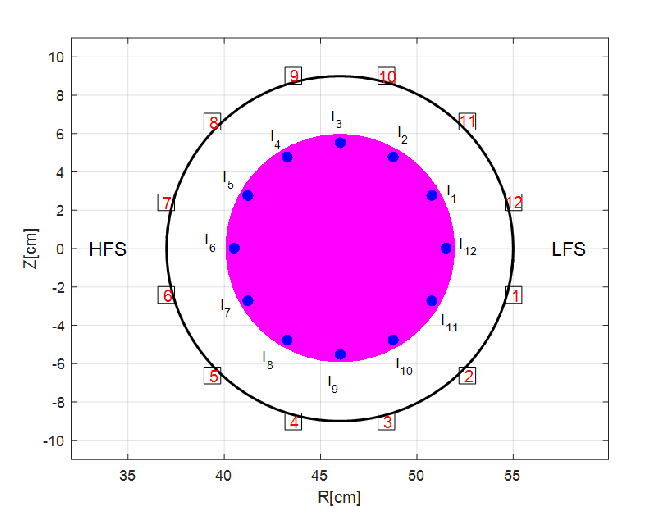
\includegraphics[width=\textwidth]{Chp4/filaments_crossSection.eps}       
		\caption{\label{filaments}}
	\end{subfigure}
	~
	\begin{subfigure}[b]{0.45\textwidth}
		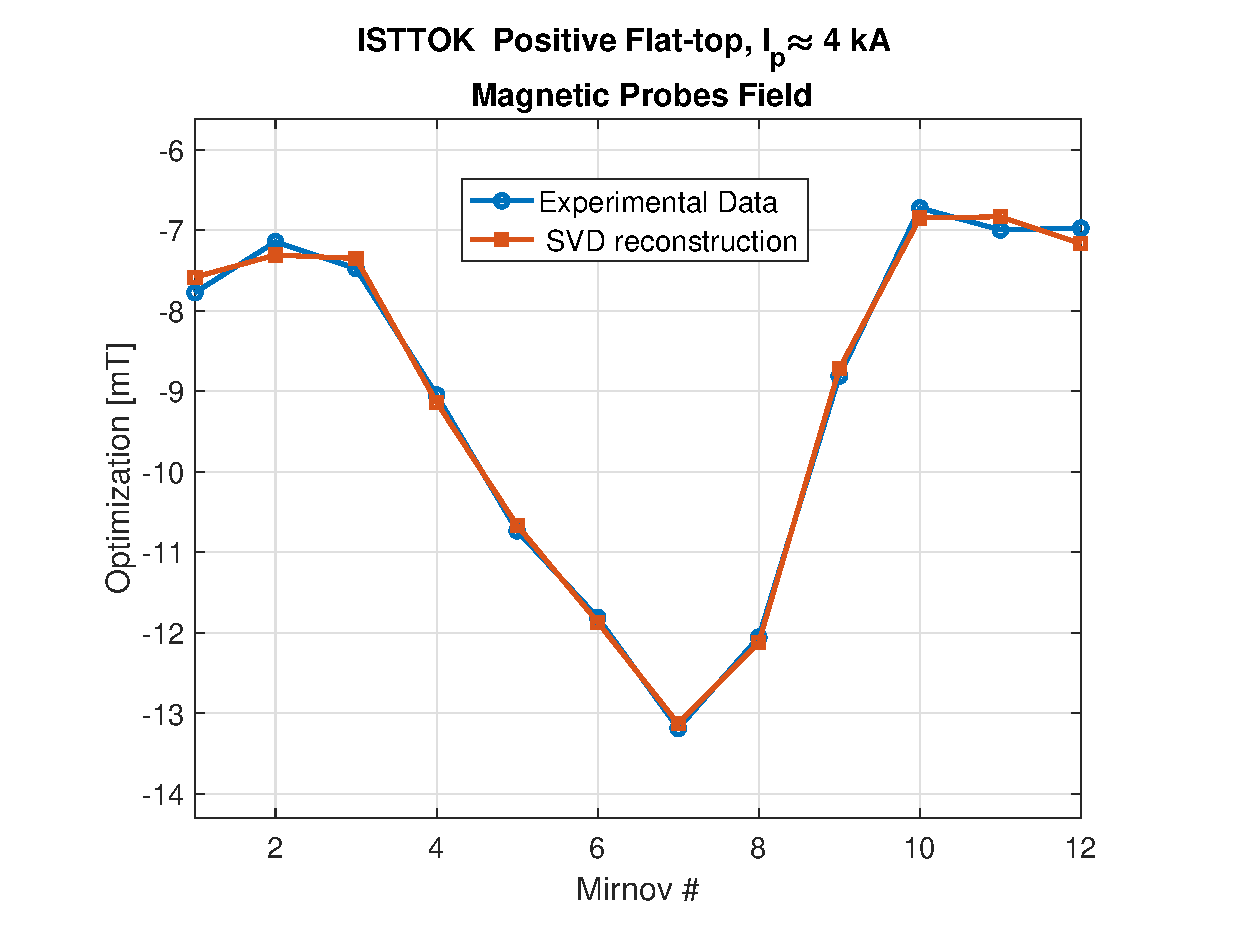
\includegraphics[width=\textwidth]{Chp4/Magnetic_probes_SVD.eps} 
		\caption{\label{fig:SVDmagn} }
	\end{subfigure}
	
	\caption{Fig.~\ref{filaments}:  ISTTOK Poloidal Cross Section with depiction of the radial and poloidal positions of the selected filaments for the plasma modelling and the magnetic probes. Fig.~\ref{fig:SVDmagn}: Comparison between magnetic probes measurements (blue line) and reconstructed values (orange line) during a plasma current positive Flat-top. }
	
\end{figure}


Afterwards it is possible to evaluate the results by comparing the magnetic measurements with the ones obtained using the filamentary currents, as in Fig.~\ref{fig:SVDmagn}; another estimation of the results is the total current in the filaments, which is approximately  equal to the total current calculated by the sum from the magnetic probes measurements (Ampere's Law) as shown in Fig.~\ref{sumIfil} . Finally, is possible to reconstruct the position of the current centroid with a weighted average of the 12 filaments currents as in eqs.~\ref{eq:CentroidPos} where $\mu$ is the respective filament number.

\begin{subequations}\label{eq:CentroidPos}
	\begin{align}
	%\label{eq:centroid_radial}
	r_0= & \sqrt{\frac{\sum_{k=1}^\mu \, i_{p,f_k}\, r^2_{p,f_k}}{\sum_{k=1}^\mu\, i_{p,f_k}}}
	\\[11pt]
	%\label{eq:centroid_vertical}
	z_0= & \frac{\sum_{k=1}^\mu\, i_{p,f_k}\, z_{p,f_k}}{\sum_{k=1}^\mu\, i_{p,f_k}}
	\end{align}
\end{subequations}

\begin{figure}[htbp]
	\centering
	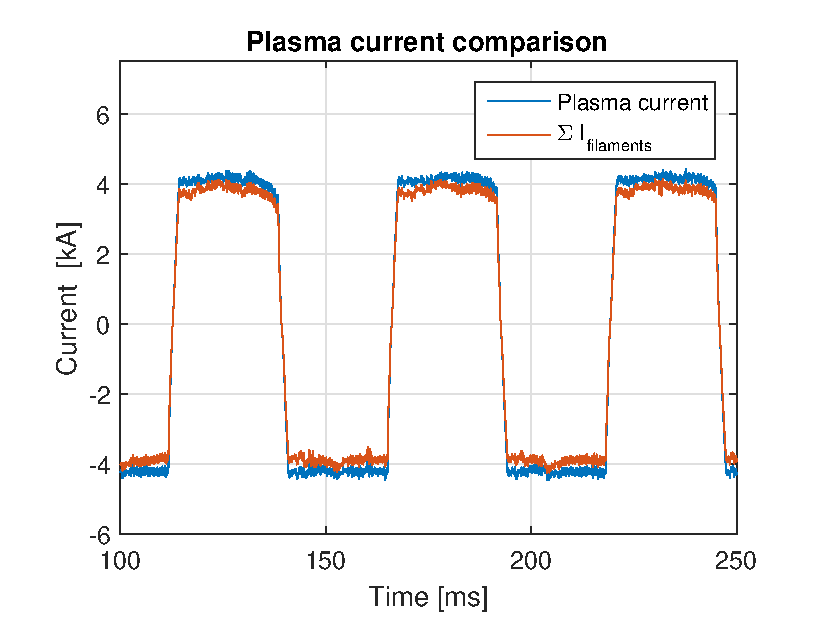
\includegraphics[,clip,width=.55\textwidth]{Chp4/Ip_sumfil.eps}
	\caption{\label{sumIfil}Comparison between the plasma current signal computed with Ampere's law  and with the  filamentary currents sum.   }
\end{figure}


\section{Real-time MARTe implementations for the plasma position reconstruction}
Real-Time control in ISTTOK relies on the execution of  Generic Application Modules (GAM) executed on MARTe ~\cite{Neto2010}. Algorithms for the subtraction of the magnetic contributions of the PF coils from the magnetic probes signals and for the reconstruction of the current centroid position were implemented in C++ language in  an specific ISTTOK GAM .

\label{implemnt}


\subsection{Poloidal magnetic external contributions subtraction}

Figure \ref{GAM_fluxes} compares the time response in one of the magnetic probes to the one reconstructed by the state-space models. During this plasma-less discharge positive and negative  current step functions waveforms  were applied at different starting times on the PF coils. In figure \ref{GAM_extfluxes} are shown the signals related to the  external fluxes subtraction on real-time  from a magnetic probe signal during a plasma current flat-top.\smallskip

\begin{figure}[h]
	\centering
	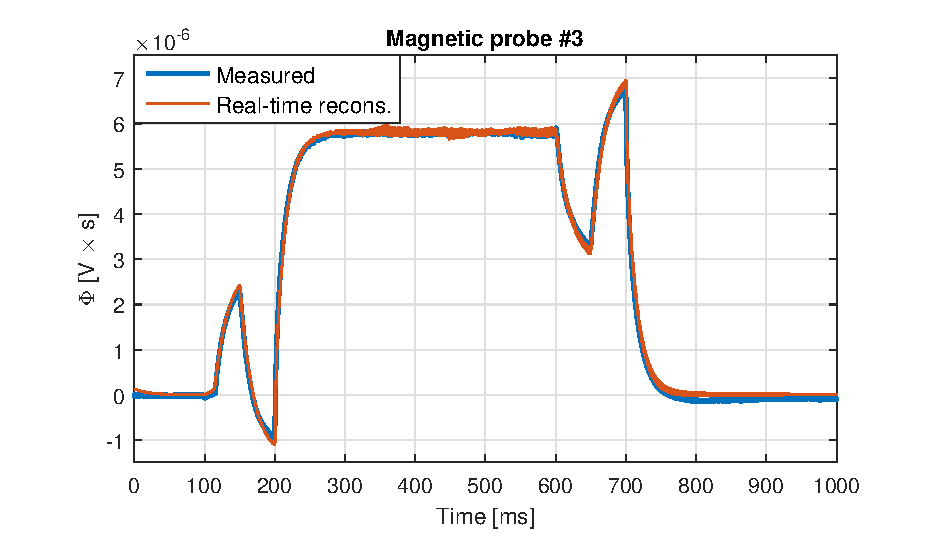
\includegraphics[,clip,width=.66\textwidth]{Chp4/GAM_compar_mirn3.eps}
	
	\caption{\label{GAM_fluxes} Real-Time reconstruction of the external fluxes contribution to the magnetic probes, this plot corresponds to the time trace of the magnetic probe $\#~3$.  }
\end{figure}

\begin{figure}[h]
	\centering
	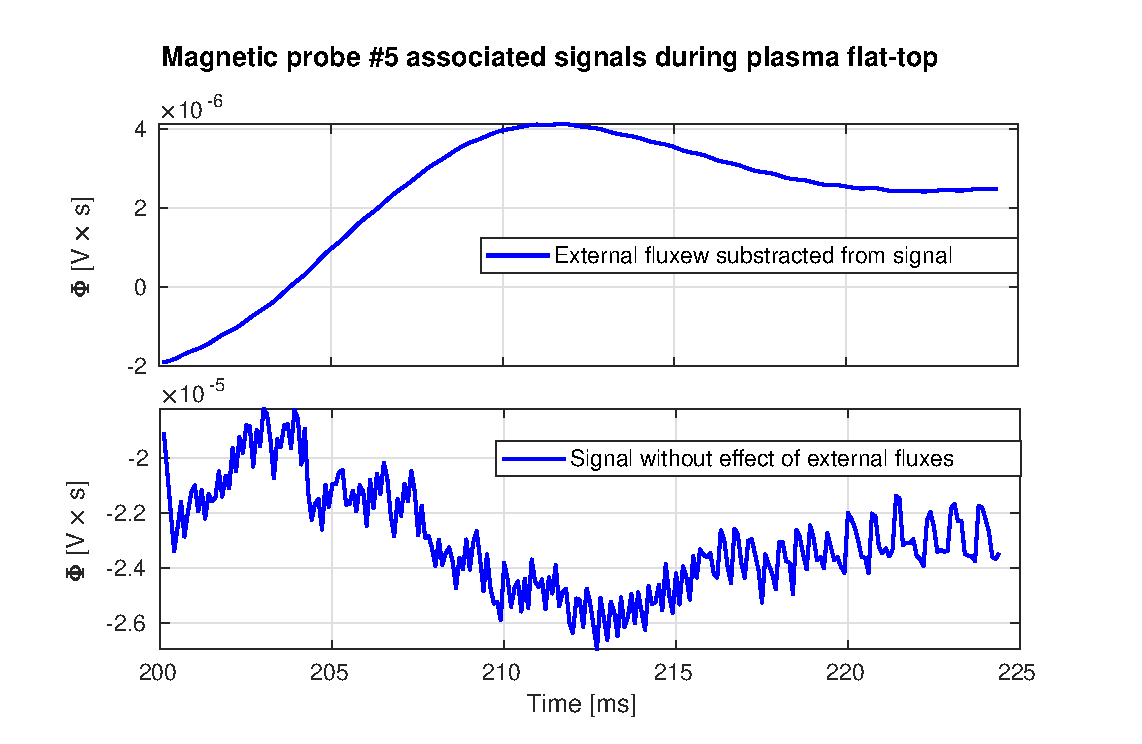
\includegraphics[,clip,width=.66\textwidth]{Chp4/ext_flux.eps}
	
	\caption{\label{GAM_extfluxes} Real-Time reconstruction during a plasma flat-top of the external fluxes  and its subtraction from the  magnetic probe signal.  }
\end{figure}
\subsection{Plasma current and  centroid position reconstruction}

In addition to the centroid position, the plasma current is also estimated in ISTTOK from the magnetic probes measurements and  programmed on top of MARTe as a discretization of Ampere's law (see eqs.~\ref{Ip})
\begin{subequations}
	\label{Ip}
	\begin{align}
	\oint_S{B \cdot dl}=&\mu_0 \,I_{plasma} \quad ,
	\\[5pt]
	\frac{2\pi r_{probe}}{N} \enspace \sum^{N=12}_{N=1} B_{probes_i}  =&\mu_0 \,I_{plasma} \quad .
	\end{align}
\end{subequations}
Figure ~\ref{mirnv1} depicts a comparison between the plasma current contribution to the magnetic Probe \# 1 and the reconstruction of it through the relation $ f_p=M_{fp}\,i_{p,f}$. Figure~\ref{RealTimePos} shows the horizontal and vertical positions and plasma current waveforms calculated on real-time during an AC  discharge. Due to the actual controller settings in the tokamak the radial position takes more time to reach the set point than the vertical position whose response is faster. Currently ISTTOK current centroid position reconstruction on real-time is performed based on the multi-filamentary model described on the previous section. \smallskip

In figure \ref{RealTimePos} is possible to compare  plasma current and position from two discharges. In the first one the control signals are based on a  centroid position reconstructed by Langmuir probes and in the second discharge the centroid  position is computed by the multi-filament model using magnetic probes. It is possible to observe  successful inversions of plasma current when the centroid is computed by the multi-filament model in comparison with the absence of plasma current inversions when computing the centroid using the Langmuir probe signals. The plasma current inversion success percentage using algorithm reconstruction assisted by  Langmuir probes in ISTTOK is $\sim 80\%$  and assisted by magnetic probes is $\sim 99.8\%$. \smallskip
\begin{figure}[h]
	\centering
	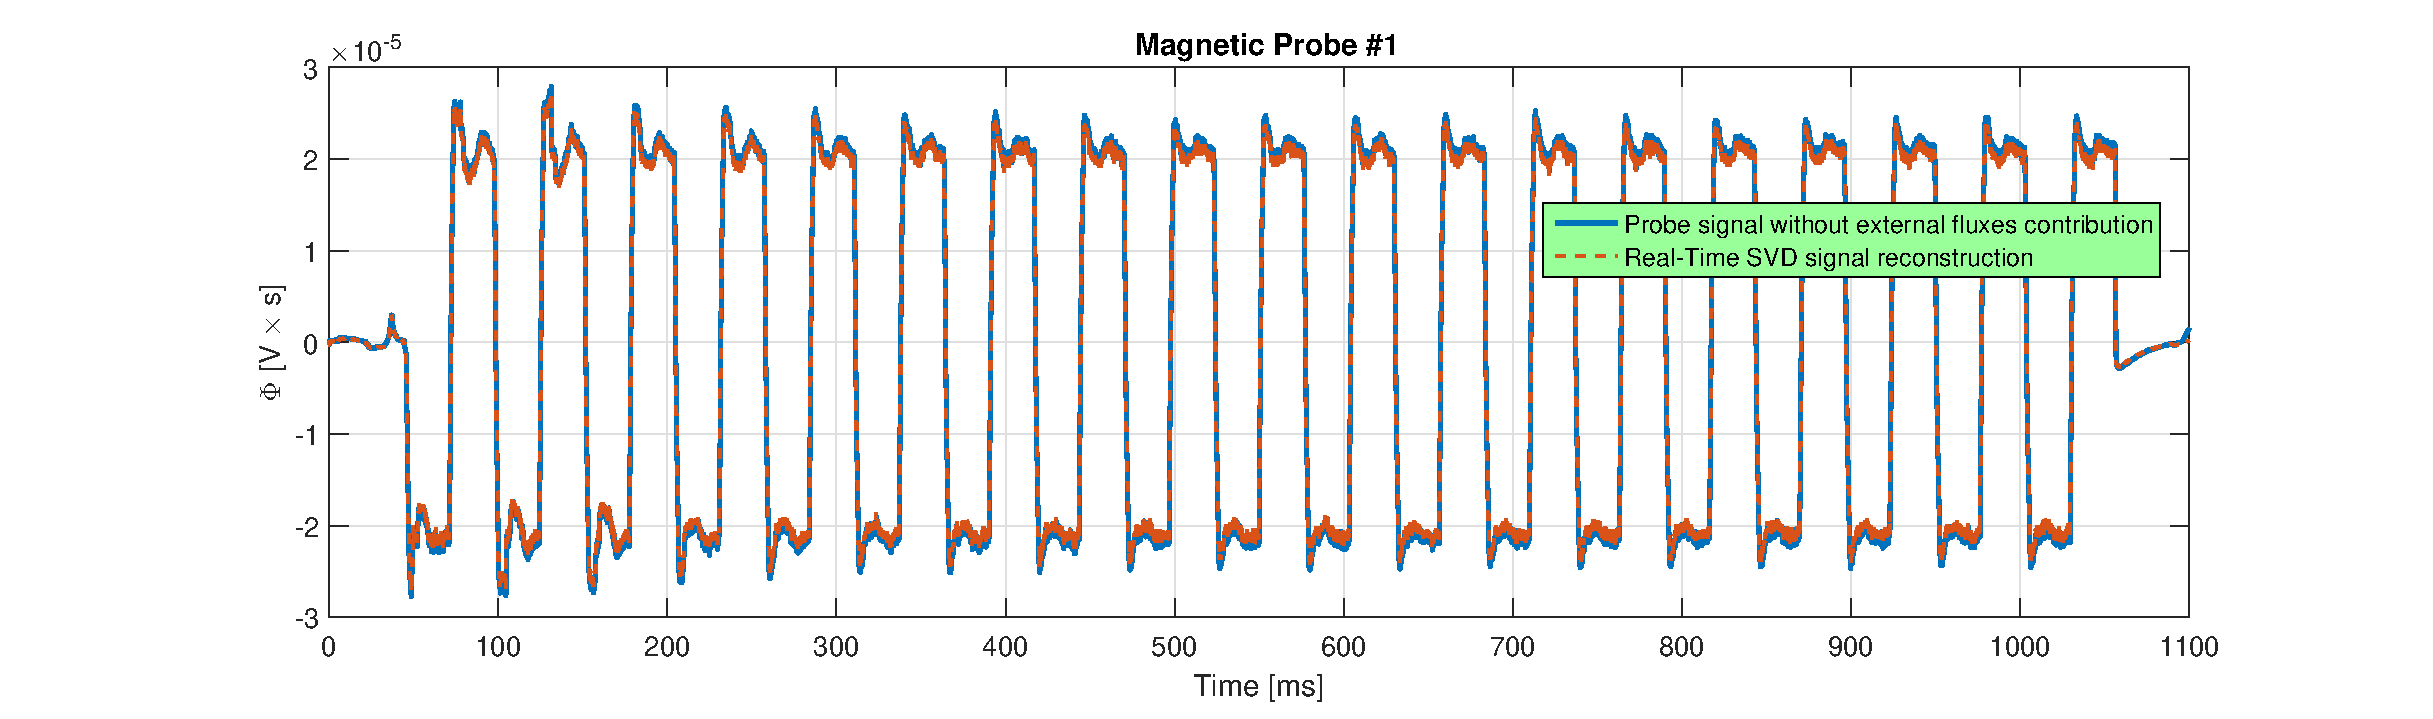
\includegraphics[width=1.1\textwidth]{Chp4/Mirnv1_comparsion.eps}
	\caption{\label{mirnv1} Comparison of the magnetic probe \# 1 signal without the contribution of the external fluxes and its real-Time SVD reconstruction over the course of an AC Plasma discharge }
\end{figure}




\begin{figure}[h]
	\centering
	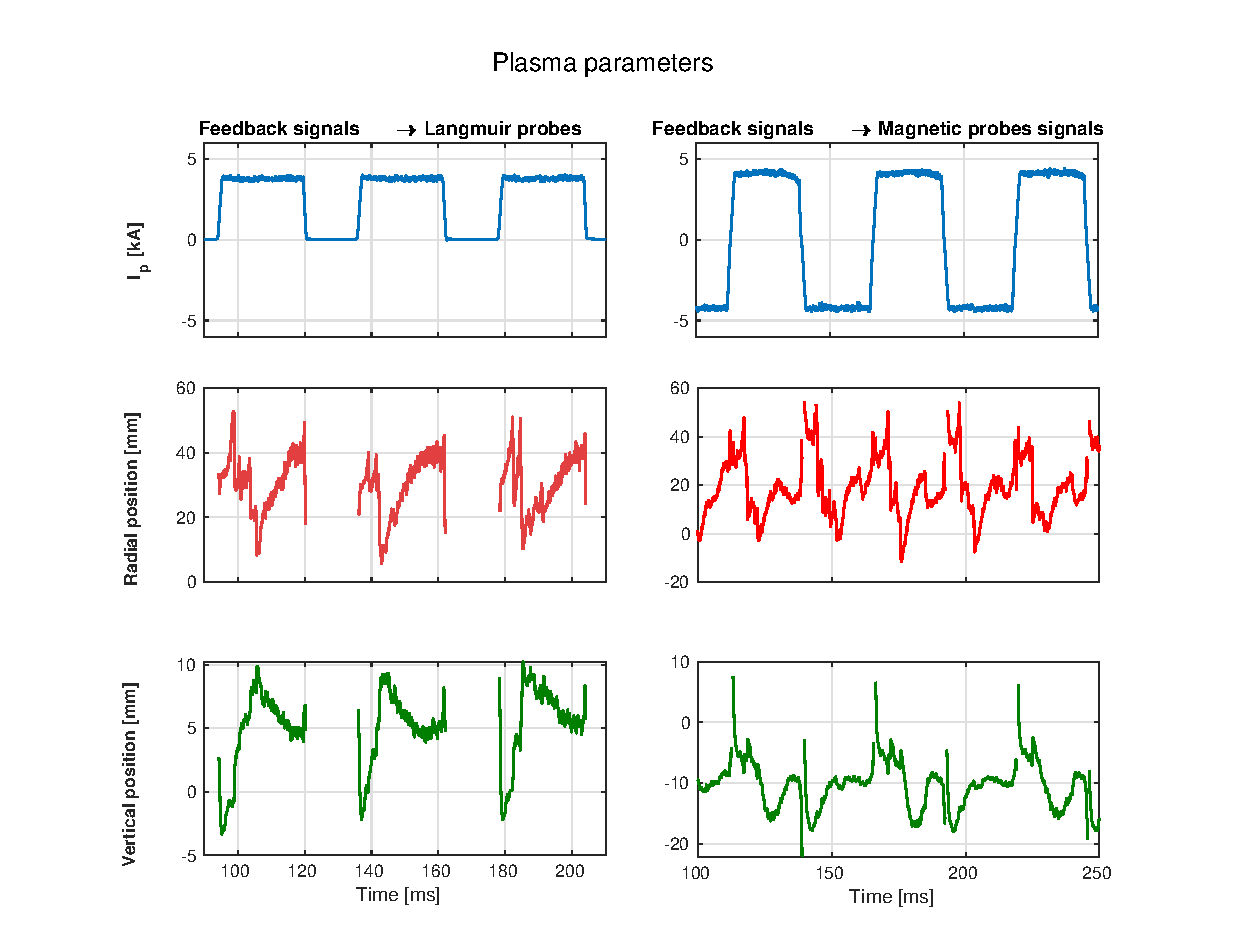
\includegraphics[width=.9\textwidth]{Chp4/Ip_R0_z0.eps}
	\caption{\label{RealTimePos}  Real-time reconstruction of the  vertical and horizontal current centroid position and plasma current  assisted by the magnetic probes signal acquisition and post-processing of two plasma discharges. Left column shows the resulting signals when the discharge control feedback is performed using Langmuir probes and right column shows when using Magnetic probes signals. Negative plasma cycles are lost when using Langmuir probes signals.    }
\end{figure}

During the realization of the work corresponding to this chapter a comprehensive analysis and processing of the ISTTOK magnetic diagnostics was done in order to obtain a reliable reconstruction of the centroid position.  With the presented corrections on the numerically hardware integrated magnetic signals in ISTTOK, it is now possible to reliably control the plasma position while varying key parameters these results are presented in the next chapter.